\documentclass{article}
\usepackage{graphicx}
\usepackage{float}


\begin{document}

\title{AI Tools and Coding in CSE113}
\author{Saboor Chaudry}

\maketitle

\section{Final Exam Topics}

\subsection{Topic: Load-Store Units in GPUs}

\begin{figure}[ht]
  \centering
  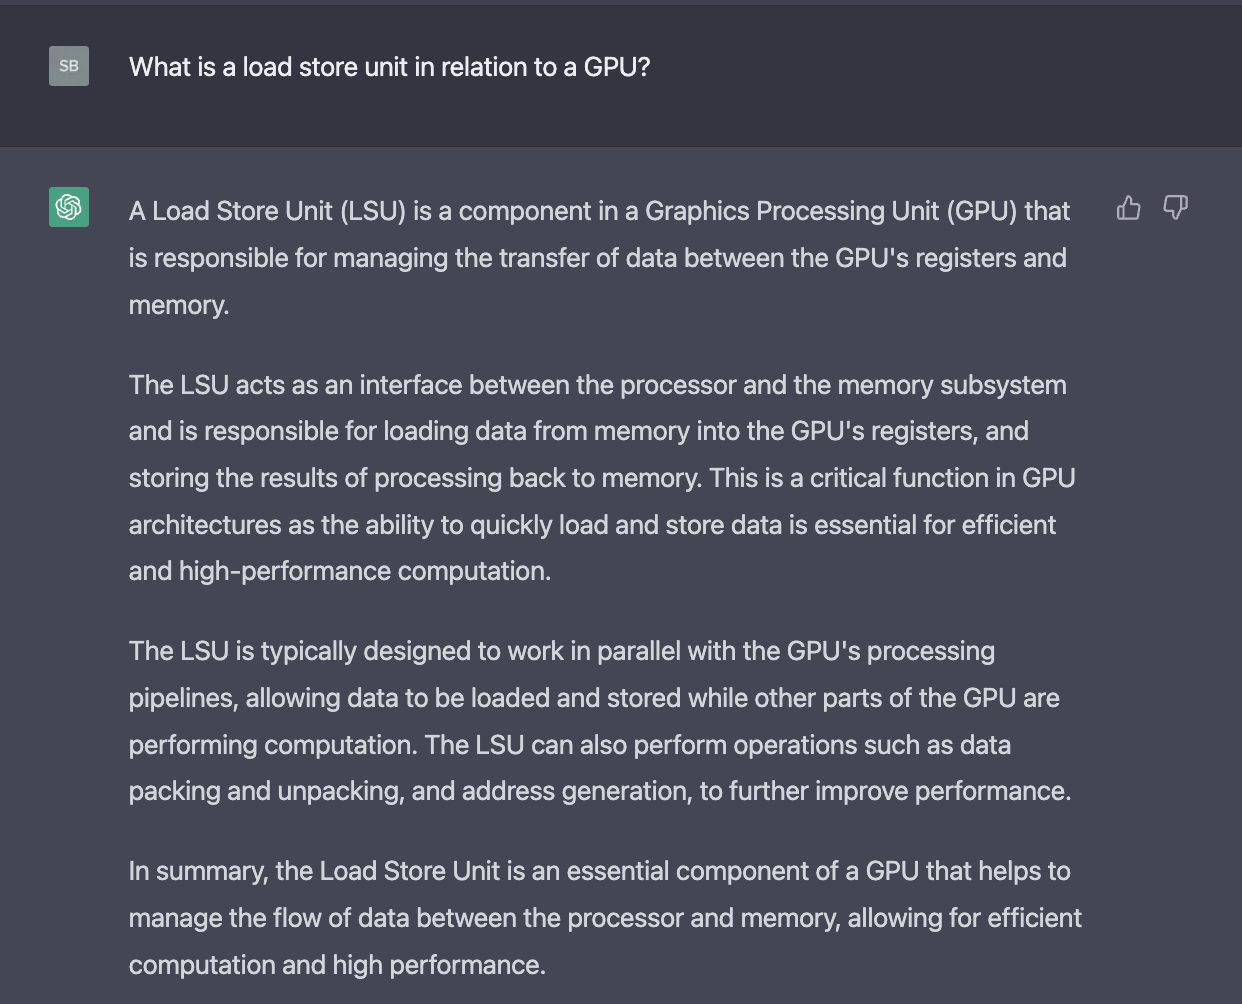
\includegraphics[width=0.9\textwidth]{loadstore.png}
  \caption{Load-Store Unit and GPU Question}
  \label{fig:loadstore}
\end{figure}

In Figure \ref{fig:loadstore}, we can see an example of a graph that can be used to represent data in Topic 1. This graph shows the relationship between X and Y variables and can be used to analyze the data.

\subsection{Topic: Semaphore Class}

\begin{figure}[H]
  \centering
  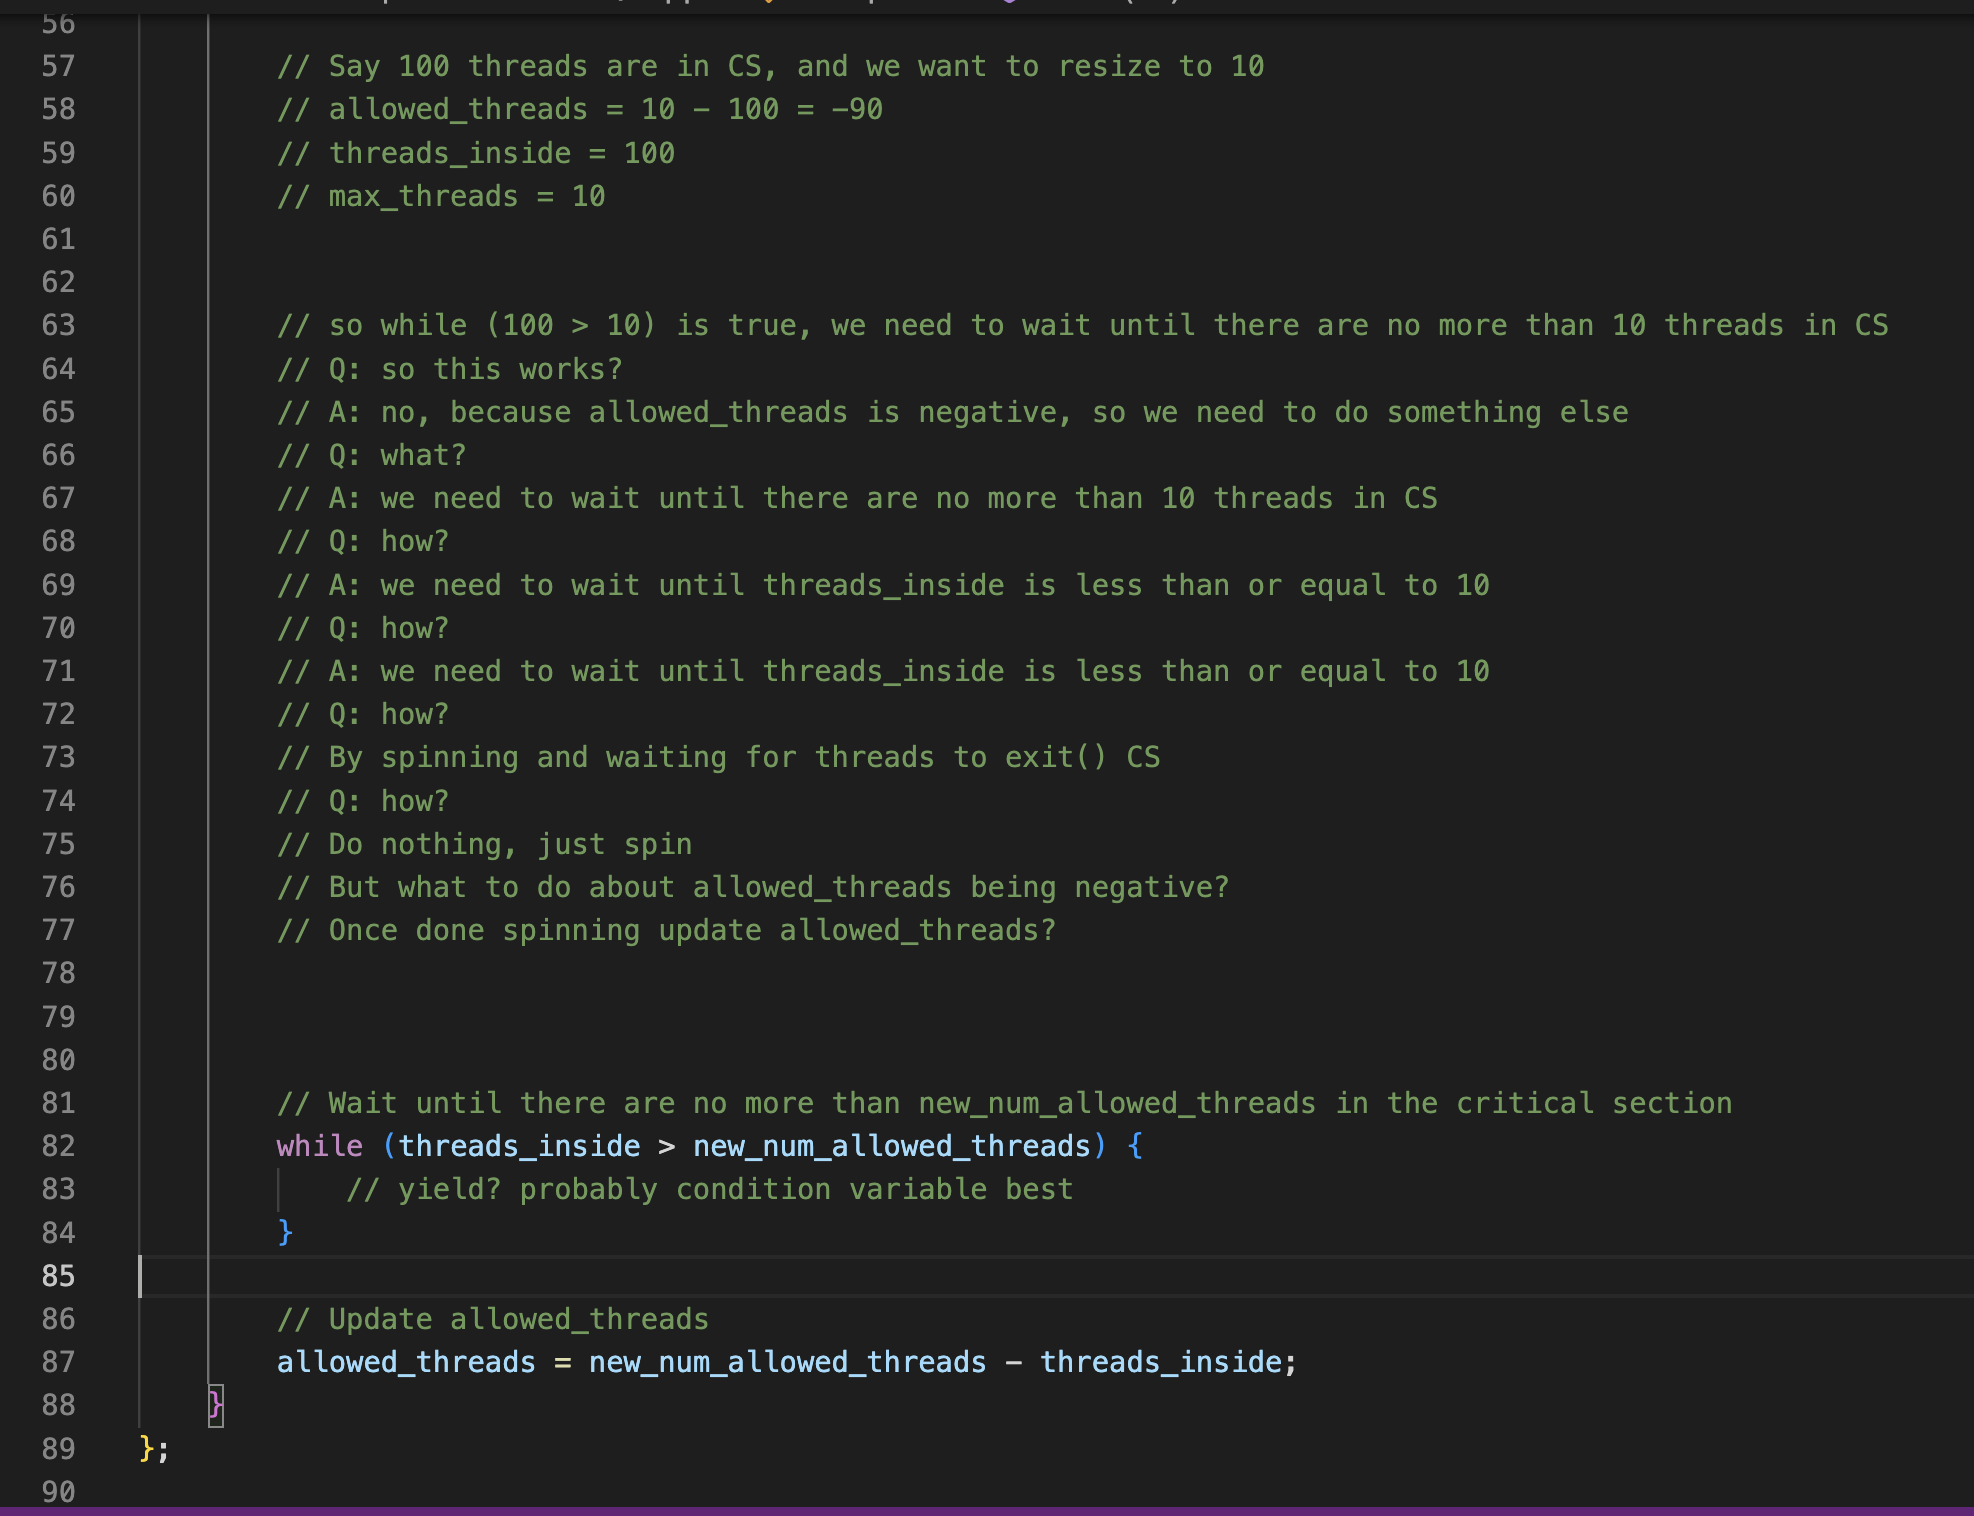
\includegraphics[width=0.95\textwidth]{semaphore1.png}
  \caption{Example image for Topic 2.}
  \label{fig:semaphore1}
\end{figure}

In Figure \ref{fig:semaphore1}, we can see an example of a decision tree that can be used to make decisions in Topic 2. This decision tree shows the different paths that can be taken based on certain conditions.


\begin{figure}[h]
    \centering
    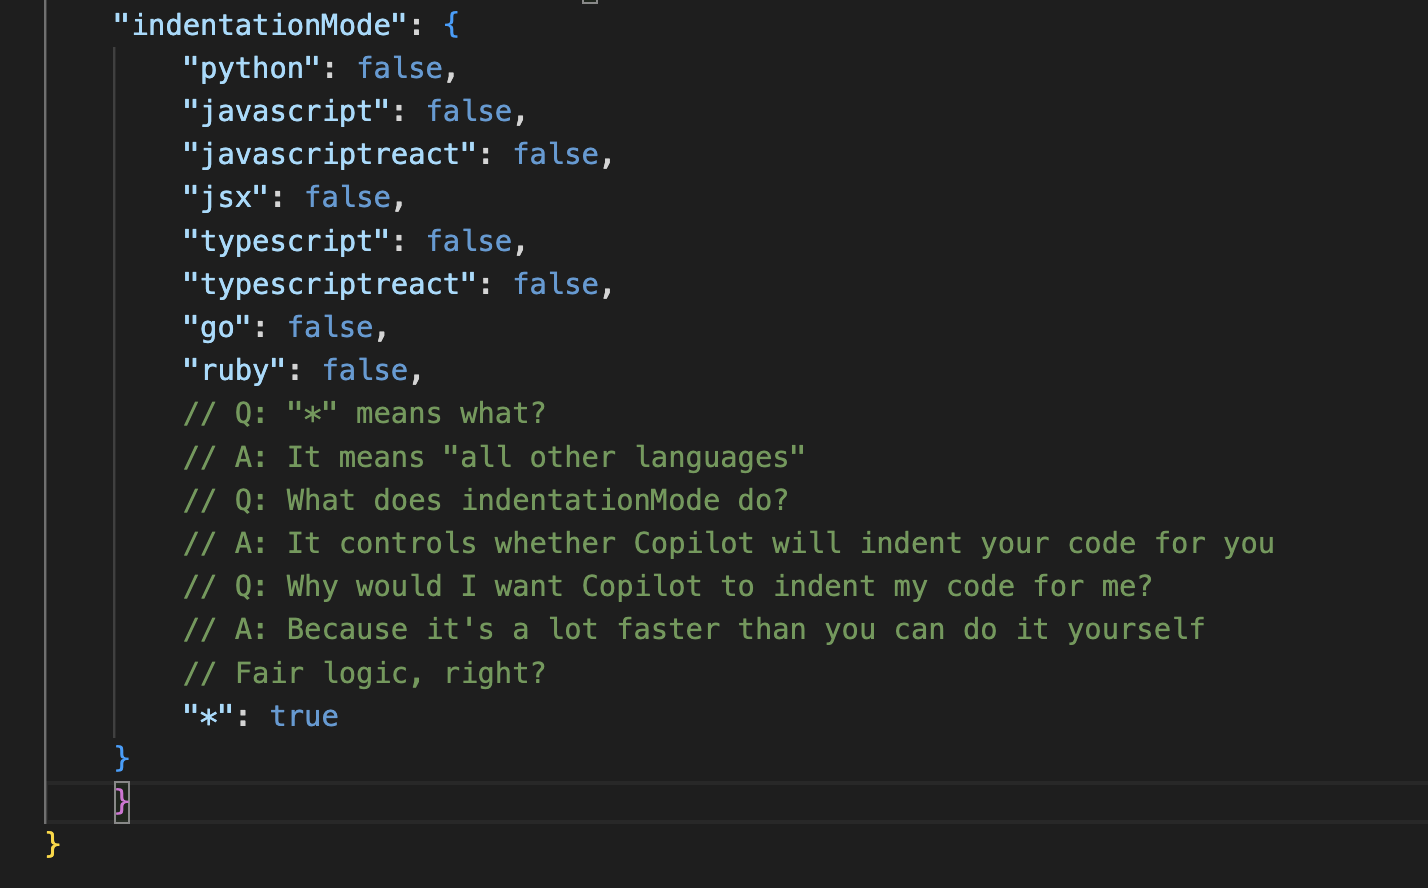
\includegraphics[width=0.5\textwidth]{image4.png}
    \caption{Caption}
    \label{fig:my_label}
\end{figure}

In Figure \ref{fig:my_label} we have semaphore continued


\subsection{Topic 3}

\begin{figure}[ht]
  \centering
  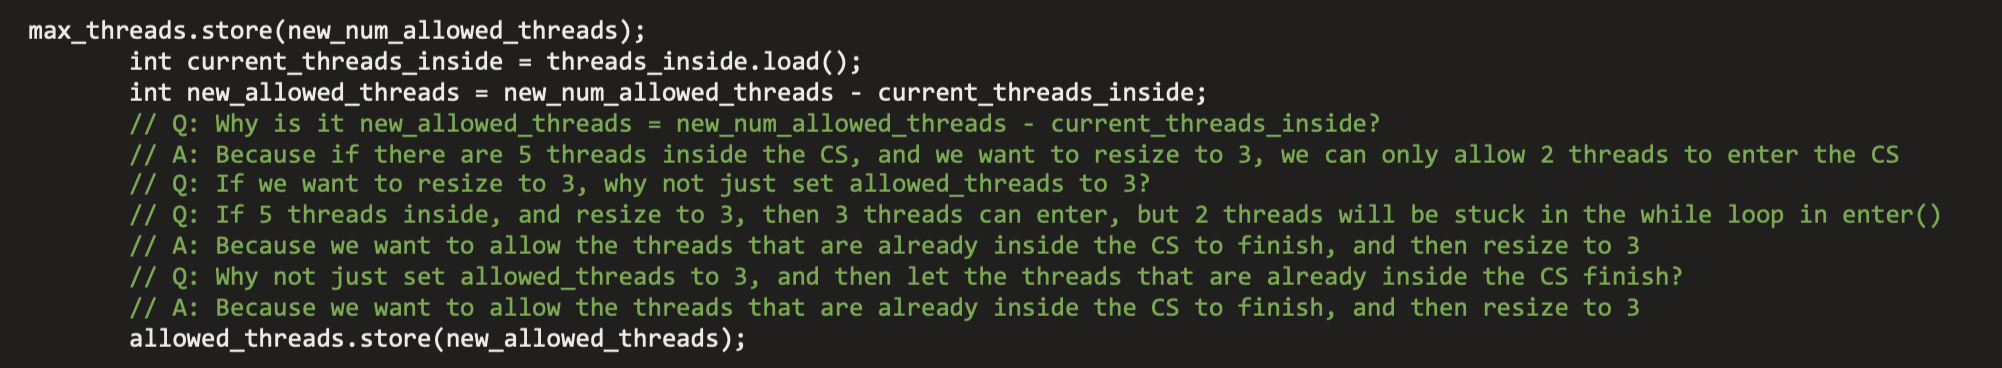
\includegraphics[width=0.95\textwidth]{semaphore2.png}
  \caption{Example image for Topic 3.}
  \label{fig:semaphore2}
\end{figure}

In Figure \ref{fig:semaphore2}, we can see an example of a neural network that can be used to classify data in Topic 3. This neural network uses layers of nodes to process data and make predictions.

\subsection{Topic 3.2}

\begin{figure}[ht]
  \centering
  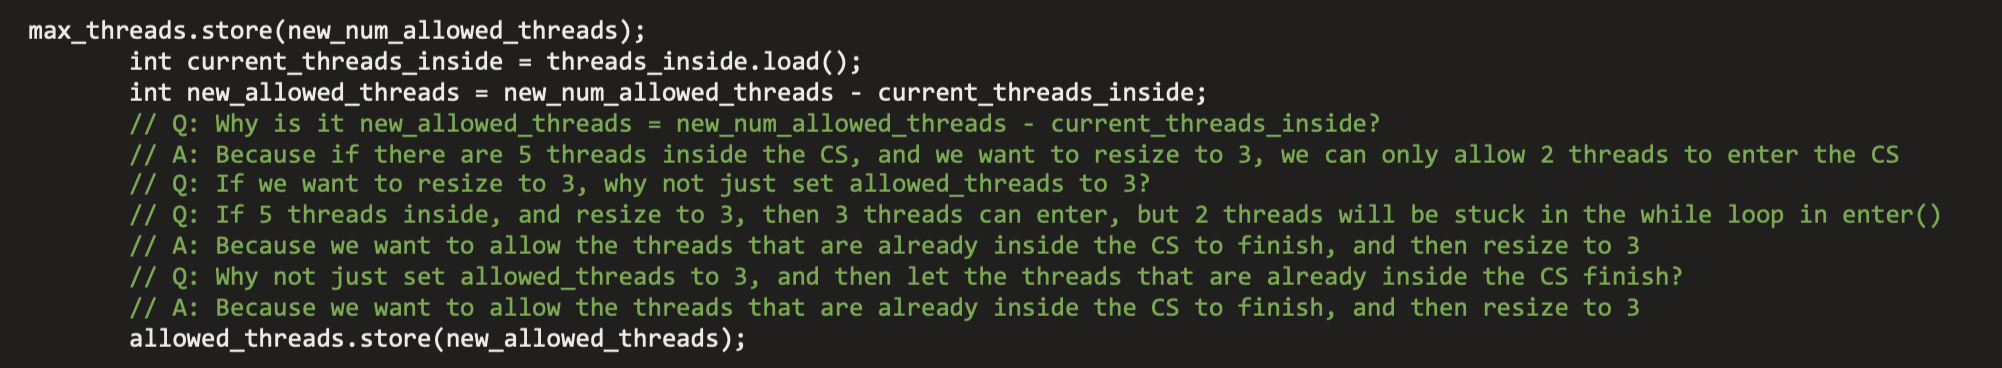
\includegraphics[width=0.95\textwidth]{semaphore2.png}
  \caption{Example image for Topic 3.2.}
  \label{fig:label3.2}
\end{figure}

In Figure \ref{fig:label3.2}, we can see an example of a neural network that can be used to classify data in Topic 3.2. This neural network uses layers of nodes to process data and make predictions.

\section{Homework Topics}

\subsection{Topic 4}

\begin{figure}[ht]
  \centering
  \includegraphics[width=0.5\textwidth]{example-image-a}
  \caption{Example image for Topic 4.}
  \label{fig:topic4}
\end{figure}

In Figure \ref{fig:topic4}, we can see an example of a graph that can be used to analyze data in Topic 4. This graph shows the distribution of a certain variable and can be used to identify trends and outliers.

\subsection{Topic 5}

\begin{figure}[ht]
  \centering
  \includegraphics[width=0.8\textwidth]{example-image-b}
  \caption{Example image for Topic 5.}
  \label{fig:5.5}
\end{figure}

In Figure \ref{fig:5.5}, we can see an example of a decision tree that can be used to make decisions in Topic 5. This decision tree shows the different paths that can be taken based on certain conditions.

\subsection{Topic 6}

\begin{figure}[ht]
  \centering
  \includegraphics[width=0.5\textwidth]{example-image-c}
  \caption{Example image for Topic 6.}
  \label{fig:topic6}
\end{figure}

In Figure \ref{fig:topic6}, we can see an example of a neural network that can be used to classify data in Topic 6. This neural network uses layers of nodes to process data and make predictions.

\subsection{Topic 7}

\begin{figure}[ht]
  \centering
  \includegraphics[width=0.5\textwidth]{example-image-a}
\end{figure}

\end{document}